\documentclass[a4paper,12pt]{scrartcl}
\usepackage[utf8]{inputenc}
\usepackage[paper=a4paper,left=1.25in,right=1.25in,top=1.25in,bottom=1.25in]{geometry}
\usepackage[doublespacing]{setspace}
\setlength{\parindent}{2em}

% koma options
\addtokomafont{section}{\fontfamily{put} \selectfont} %Kapitel
\addtokomafont{sectioning}{\fontfamily{put} \selectfont} %Titelzeilen
\deffootnote{2em}{0em}{\thefootnotemark\textemdash }

% keep lines together
\widowpenalty=10000
\clubpenalty=10000
\raggedbottom


% figures
\usepackage{graphicx}

% captions
\usepackage{caption}
\captionsetup[table]{
	labelsep=period,
	justification=centering,
	format=plain,
	textfont=footnotesize,
	name=Table,
	labelfont={footnotesize, bf},
	skip=6pt,
	position=top
}
\captionsetup[figure]{
	labelsep=period,
	justification=centering,
	format=plain,
	textfont=footnotesize,
	name=Figure,
	labelfont={footnotesize, bf},
	skip=6pt,
	position=top,
	width=12cm
}
\renewcommand{\thetable}{\arabic{table}}
\renewcommand{\thefigure}{\arabic{figure}}

% links
\usepackage[colorlinks=true, citecolor=blue, urlcolor=blue, linkcolor=blue]{hyperref} %, backref=page

% metadata
\title{Example Manuscript}

\author{
    Maximilian Sprengholz \\[-15pt]
    {\small Humboldt-Universität zu Berlin}  \\[-15pt]
    {\small \href{mailto:maximilian.sprengholz@hu-berlin.de}{maximilian.sprengholz@hu-berlin.de}}
}

\date{\normalsize \today}

%%% document starts here %%%%%%%%%%%%%%%%%%%%%%%%%%%%%%%%%%%%%%%%%%%%%%%%%%%%%%%%%%%%%%%%%%%%%%%%%%%
\begin{document}
%TC:ignore
\maketitle
\thispagestyle{empty}

\newpage

% a first section
\section{Nice Plots}

% stata histogram
\begin{figure}[!ht]
	\begin{center}
		\captionof{figure}{Stata Histogram: Miles per Gallon}
        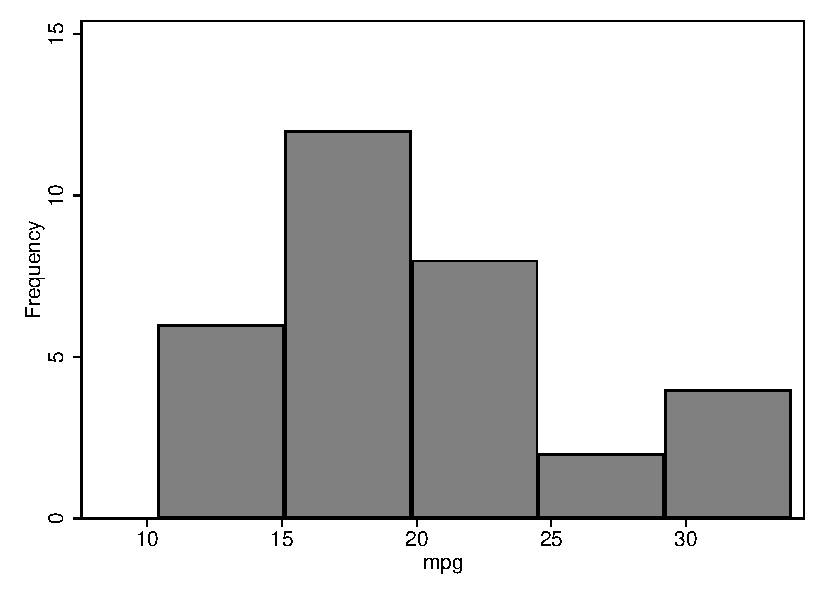
\includegraphics{../../results/figures/stata_hist_mpg.pdf}
	\end{center}
\end{figure}

% r histogram
\begin{figure}[!ht]
	\begin{center}
		\captionof{figure}{R Histogram: Miles per Gallon}
        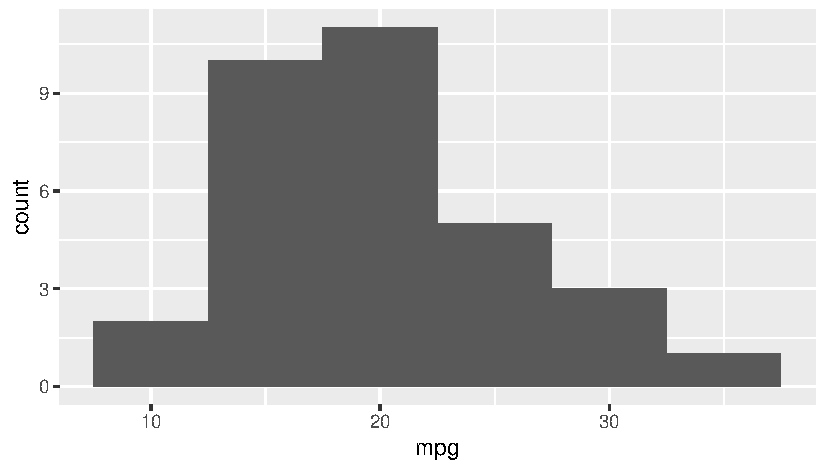
\includegraphics{../../results/figures/r_hist_mpg.pdf}
	\end{center}
\end{figure}


% a new section
\section{Nice Tables}

% stata summary table
\begin{table}[!ht]
	\begin{center}
        \captionof{table}{Stata summary table}
        {
\def\sym#1{\ifmmode^{#1}\else\(^{#1}\)\fi}
\begin{tabular}{l*{1}{ccccc}}
\hline\hline
            &       count&        mean&          sd&         min&         max\\
\hline
mpg         &          32&    20.09062&    6.026948&        10.4&        33.9\\
hp          &          32&    146.6875&    68.56287&          52&         335\\
cyl         &          32&      6.1875&    1.785922&           4&           8\\
\hline\hline
\end{tabular}
}

	\end{center}
\end{table}

% r summary table
\begin{table}[!ht]
	\begin{center}
        \captionof{table}{R summary table}
        
% Table created by stargazer v.5.2.3 by Marek Hlavac, Social Policy Institute. E-mail: marek.hlavac at gmail.com
% Date and time: Mi, Mai 17, 2023 - 07:56:26
\begin{tabular}{@{\extracolsep{5pt}}lccccc} 
\\[-1.8ex]\hline 
\hline \\[-1.8ex] 
Statistic & \multicolumn{1}{c}{N} & \multicolumn{1}{c}{Mean} & \multicolumn{1}{c}{St. Dev.} & \multicolumn{1}{c}{Min} & \multicolumn{1}{c}{Max} \\ 
\hline \\[-1.8ex] 
mpg & 32 & 20.091 & 6.027 & 10.400 & 33.900 \\ 
hp & 32 & 146.688 & 68.563 & 52 & 335 \\ 
cyl & 32 & 6.188 & 1.786 & 4 & 8 \\ 
\hline \\[-1.8ex] 
\end{tabular} 

	\end{center}
\end{table}


\end{document}